\begin{figure}[H]
    \centering
    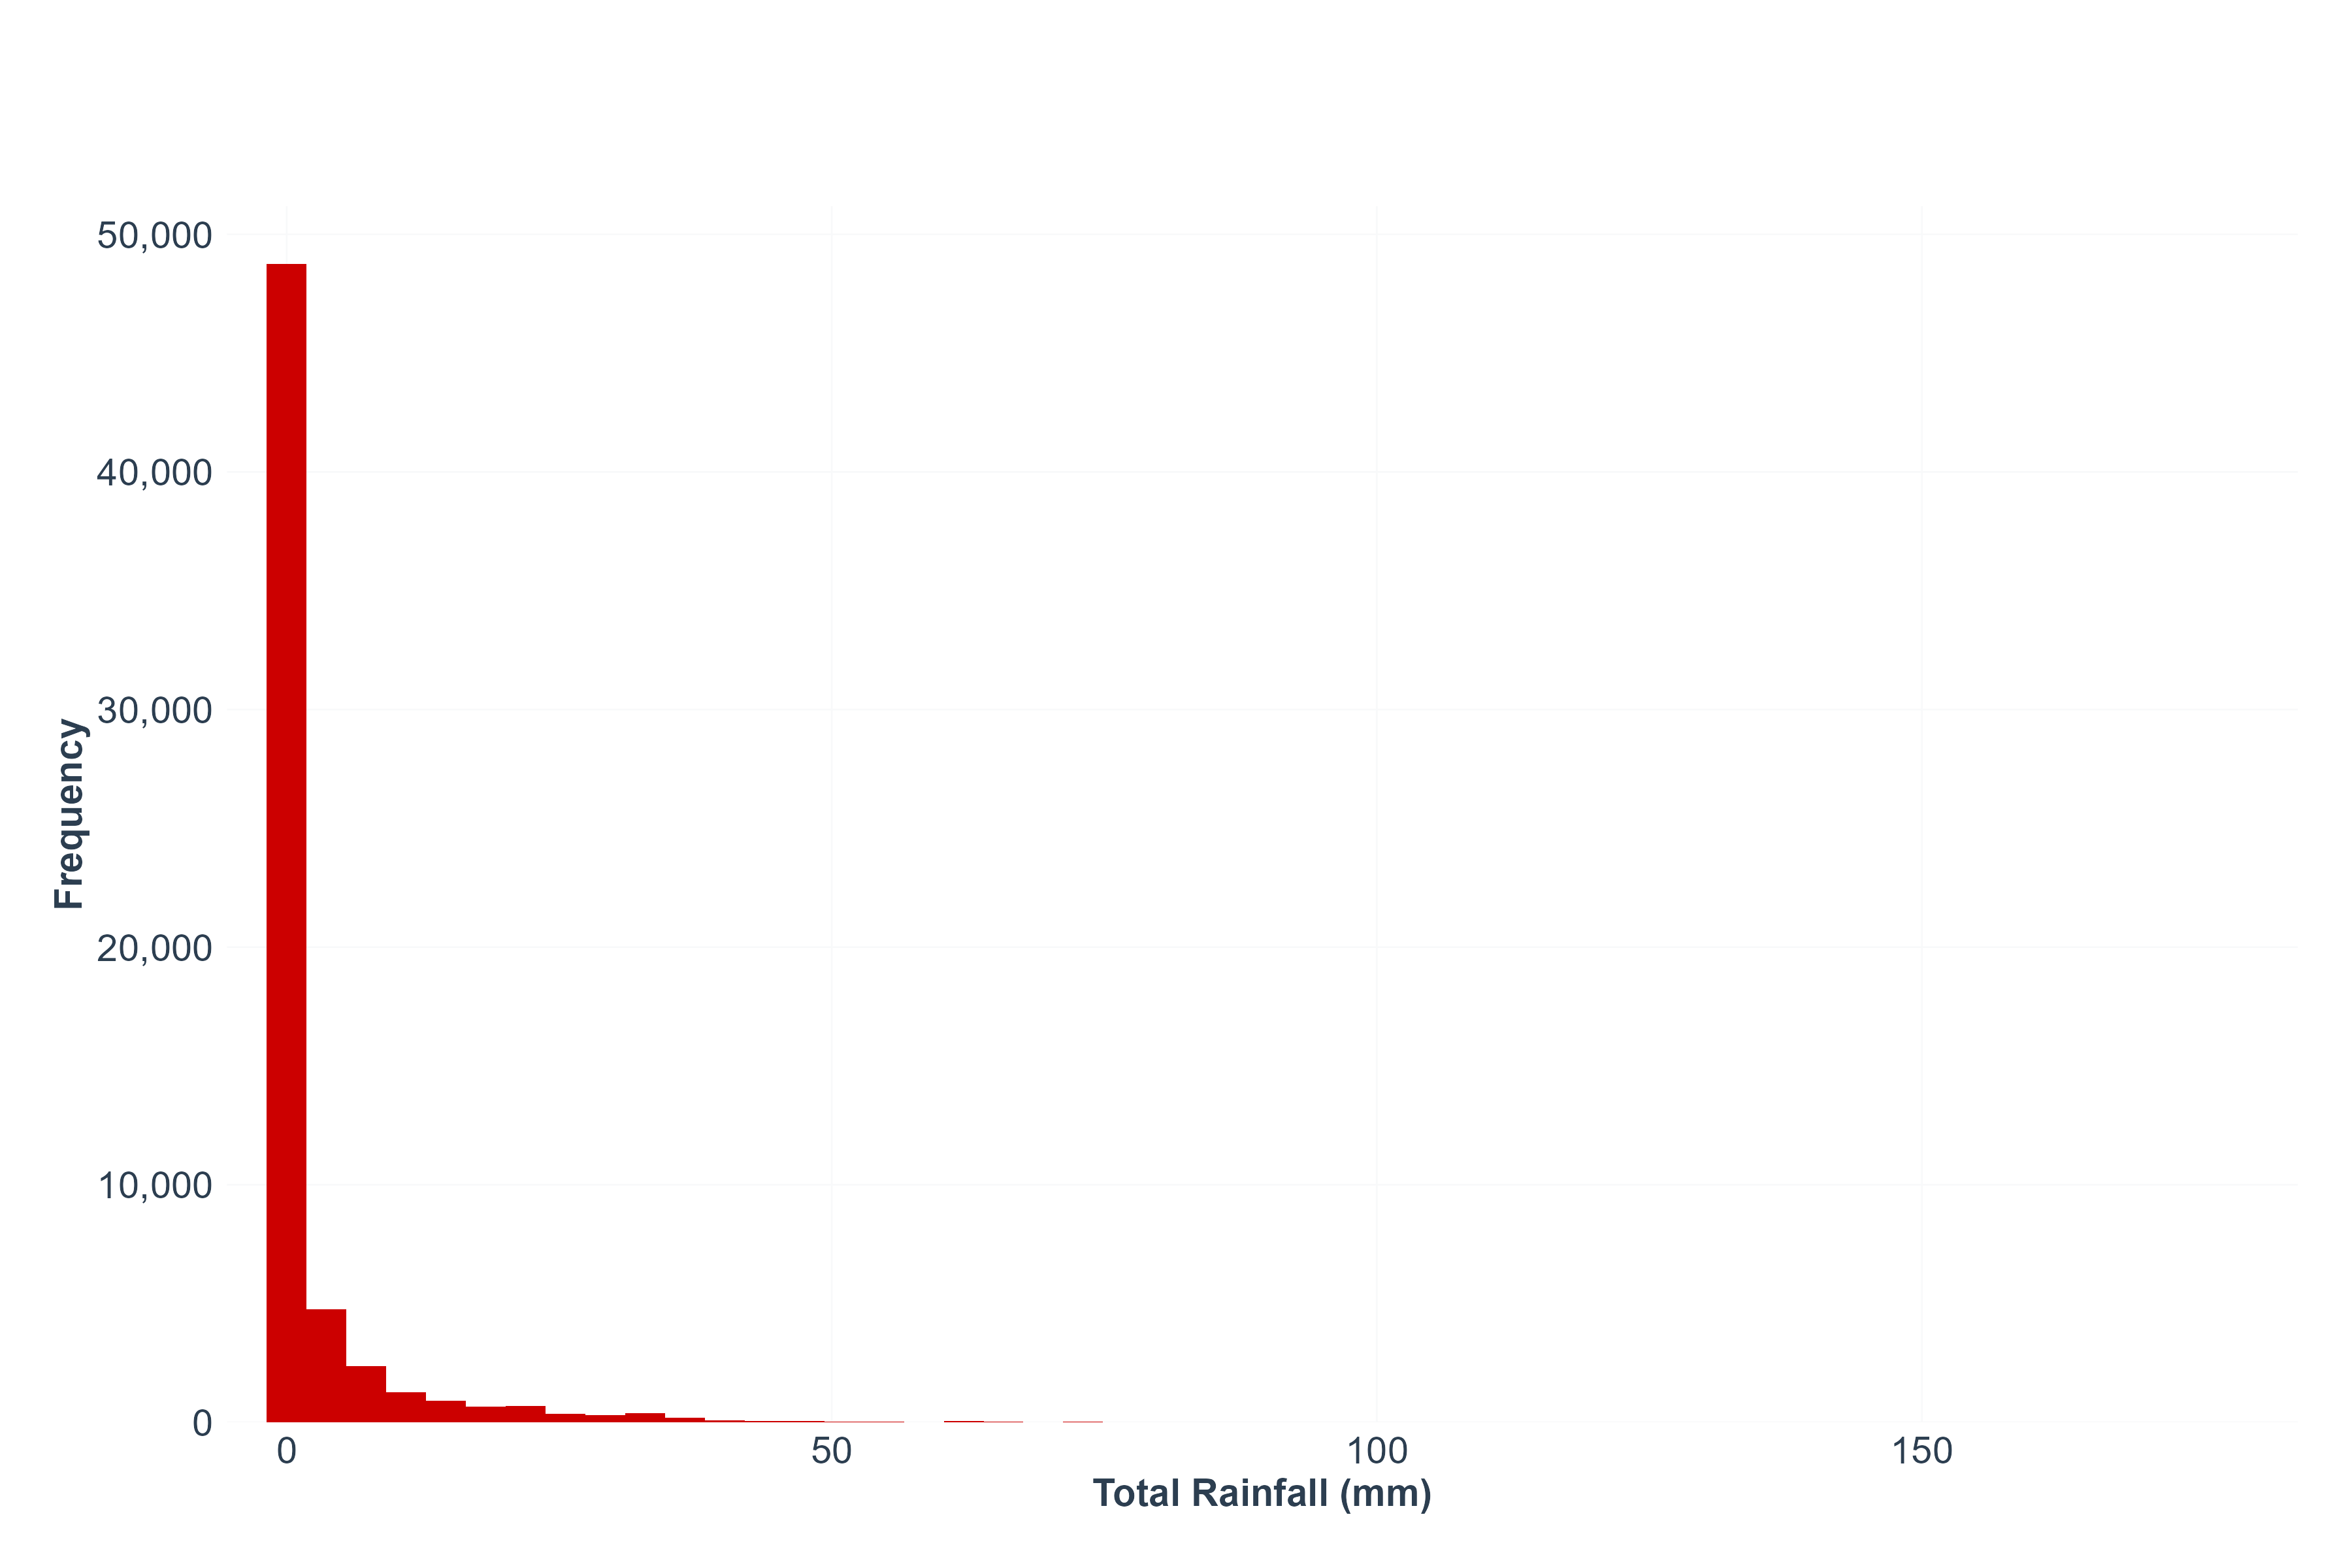
\includegraphics[width=0.5\textwidth]{../figures/rainfall_histogram.png}
    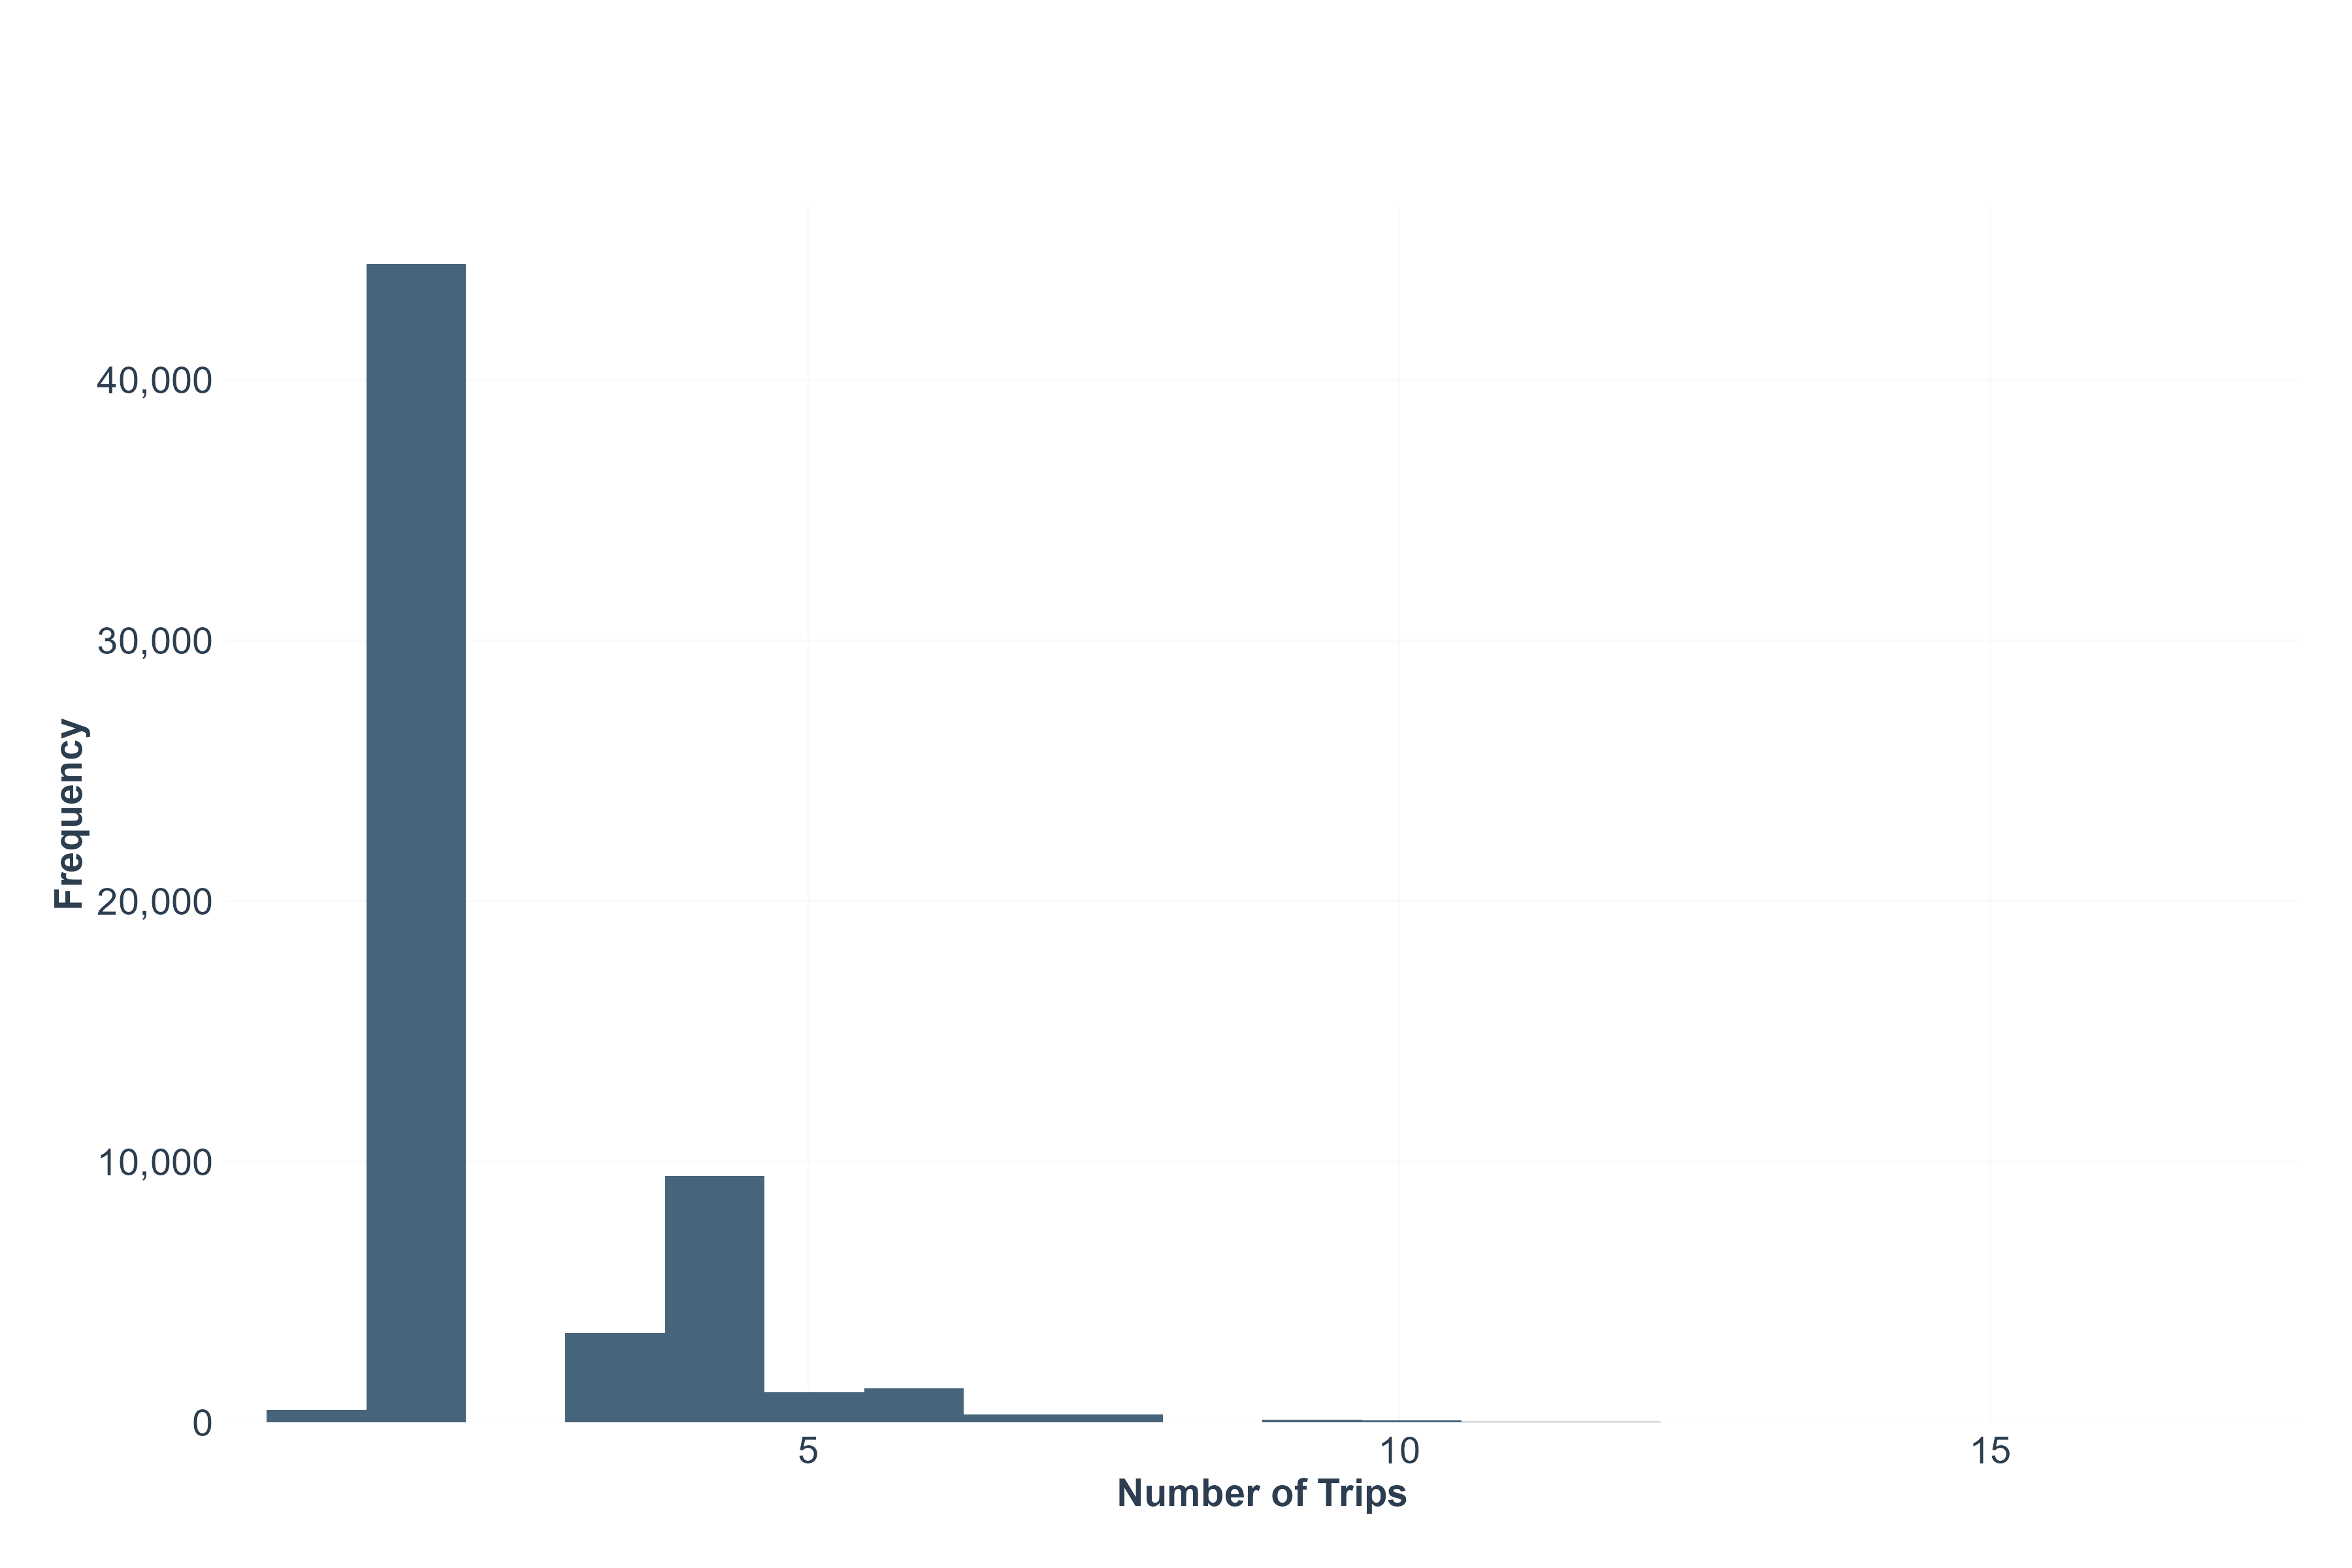
\includegraphics[width=0.5\textwidth]{../figures/trips_histogram.png}
    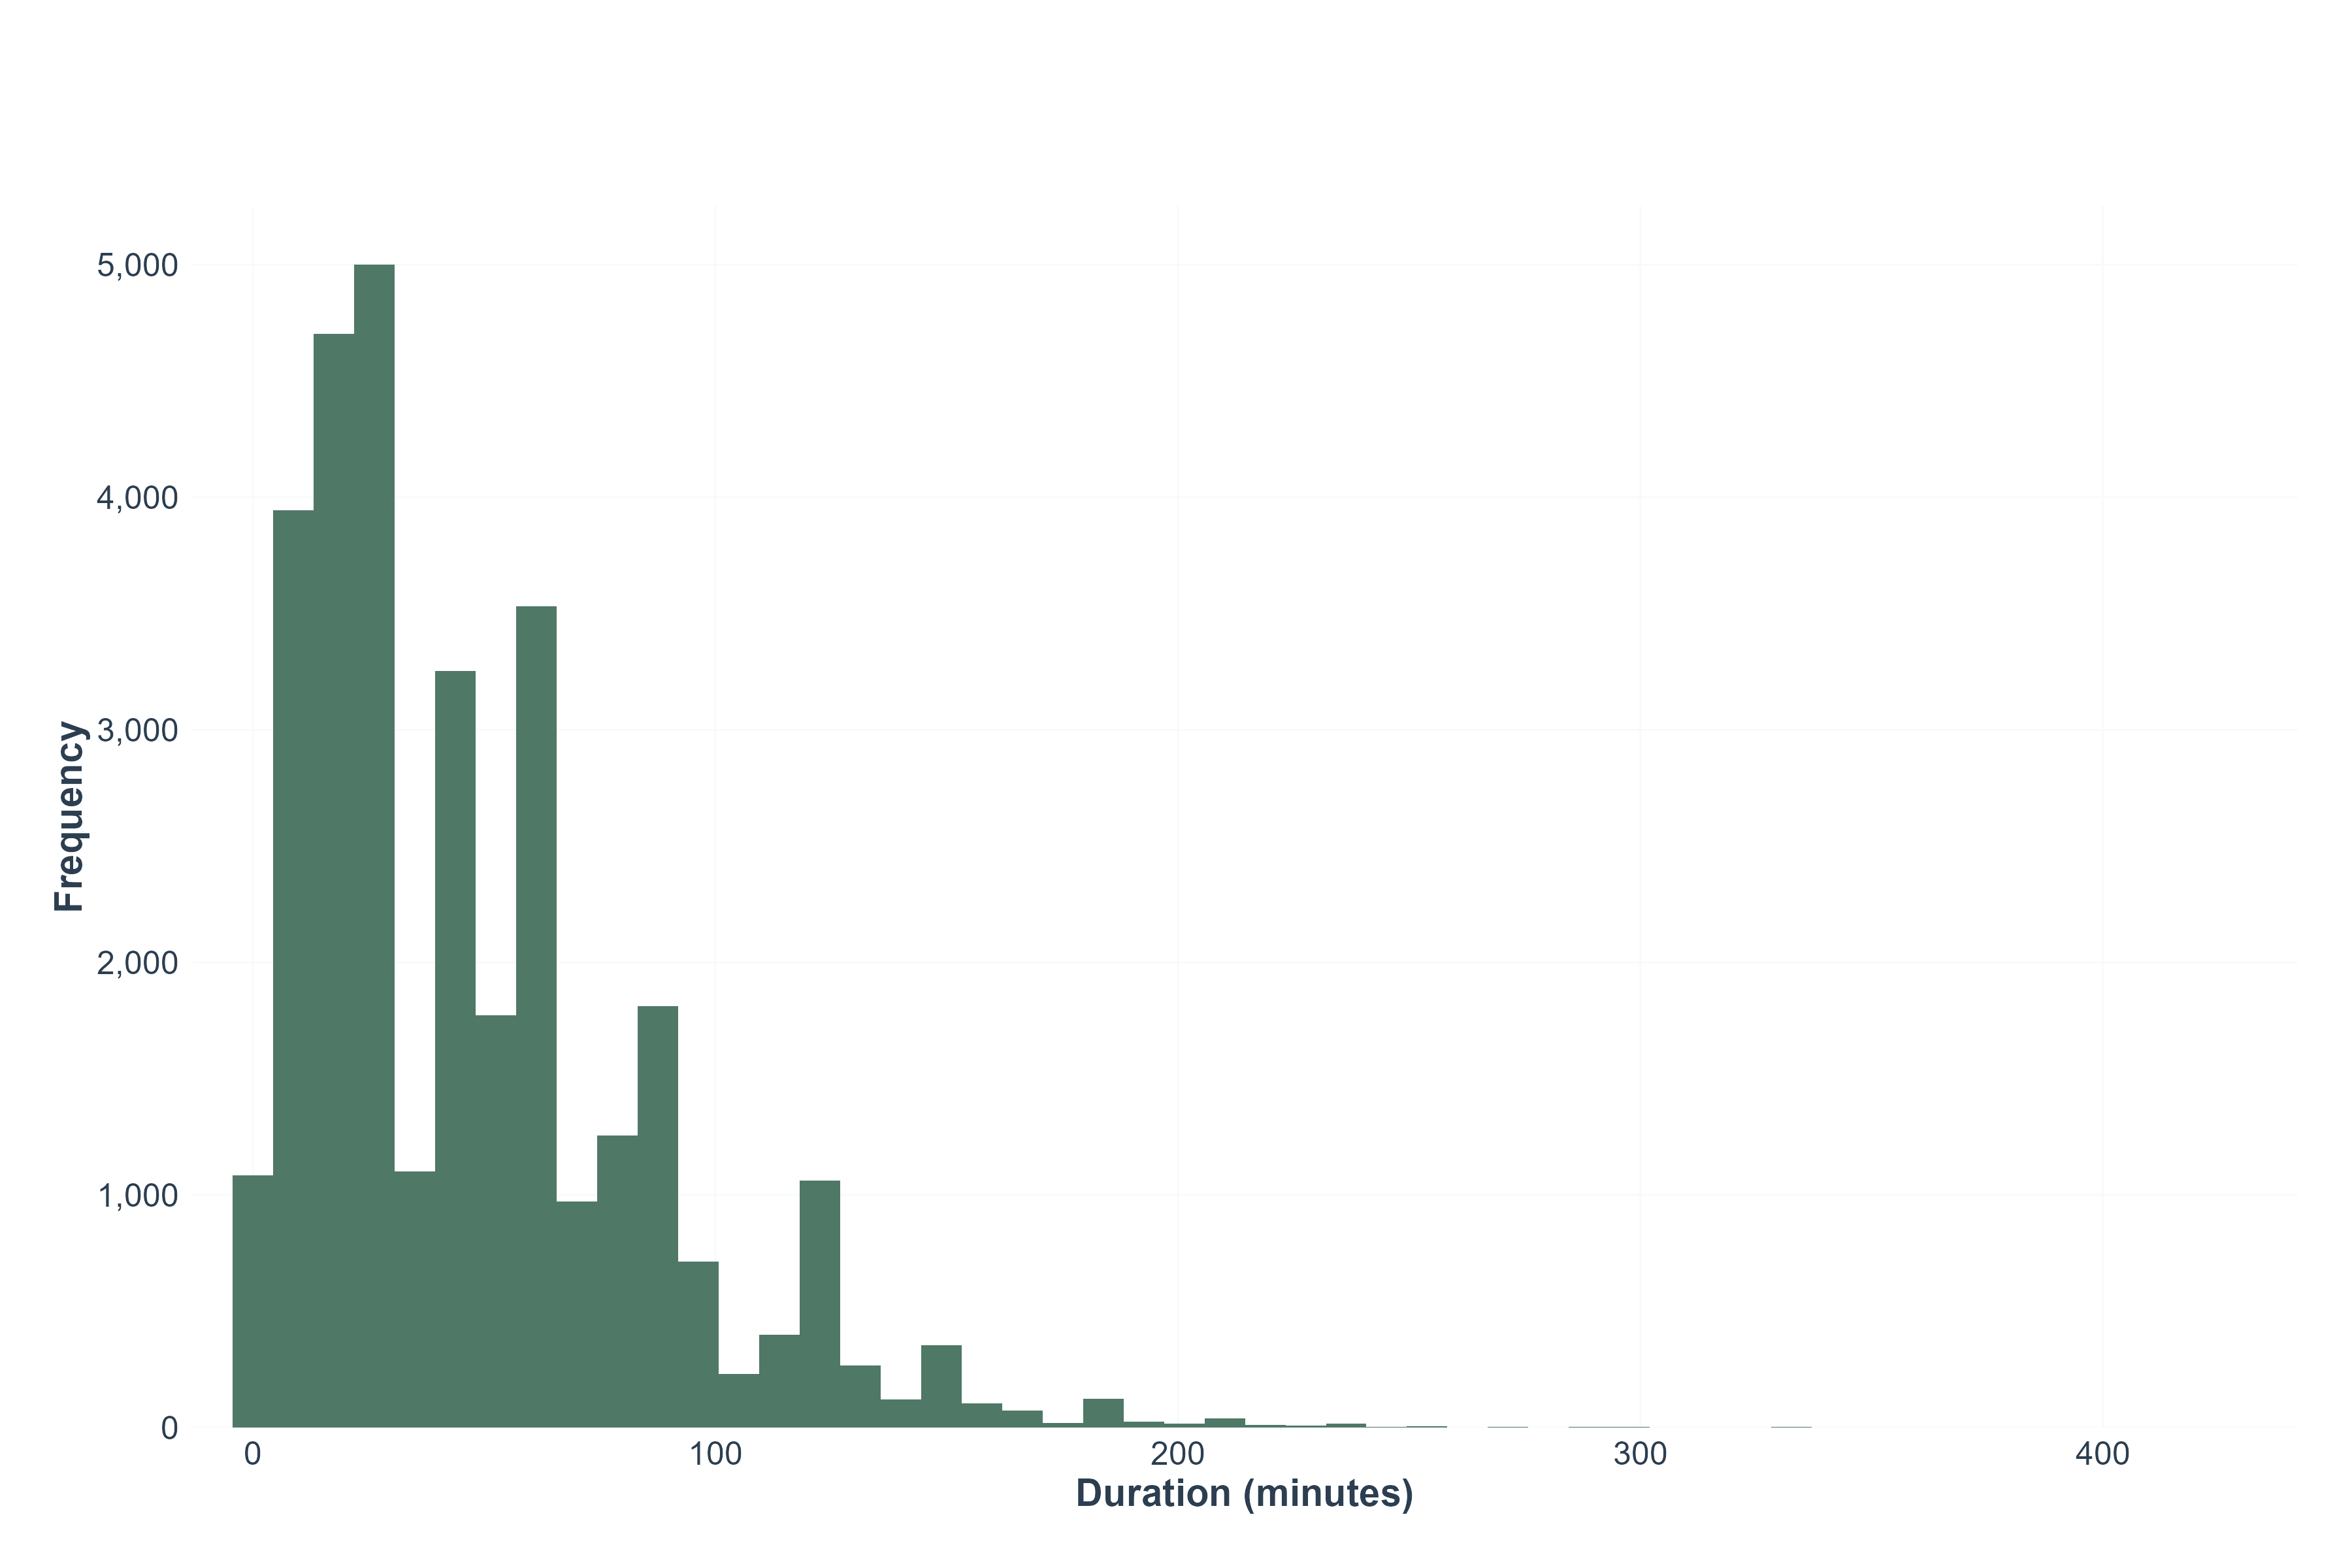
\includegraphics[width=0.5\textwidth]{../figures/duration_histogram.png}
    \caption{Histograms showing the distributions of rainfall (left), number of trips (center), and trip durations (right) in the dataset.}
    \label{fig:hist}
\end{figure}

\begin{figure}[H]
    \centering
    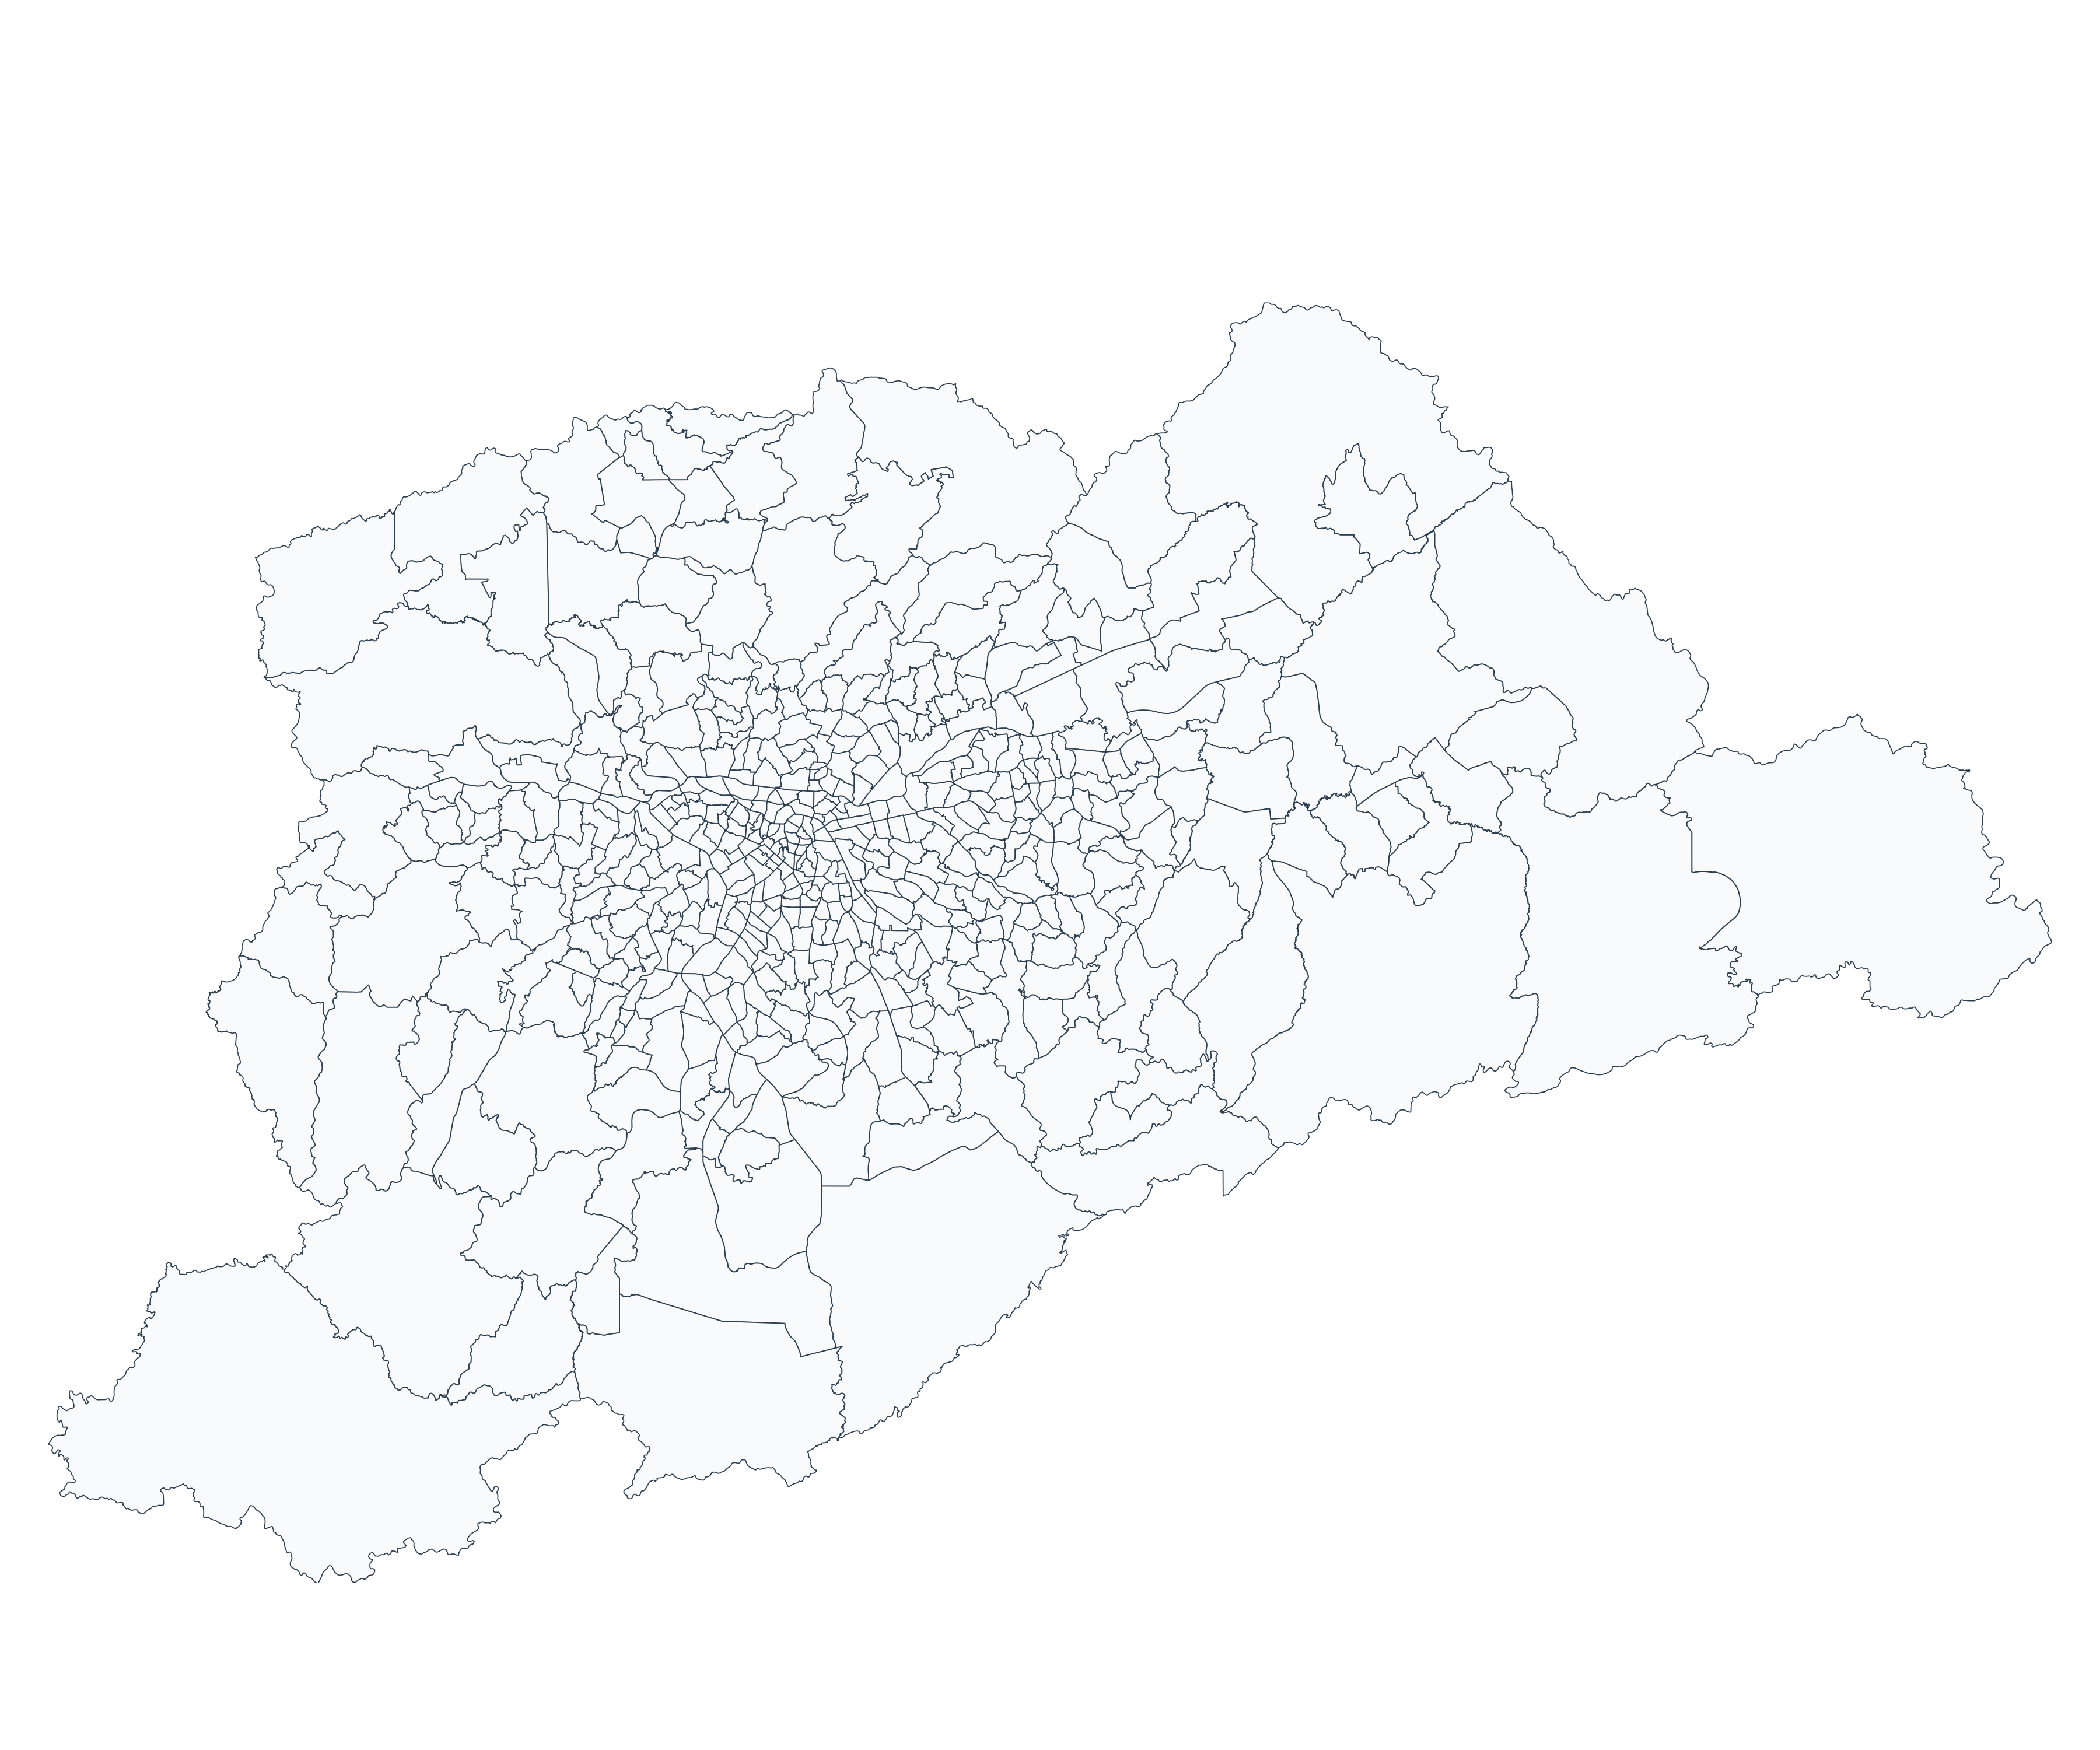
\includegraphics[width=0.45\textwidth]{../figures/rmsp_base.png}%
    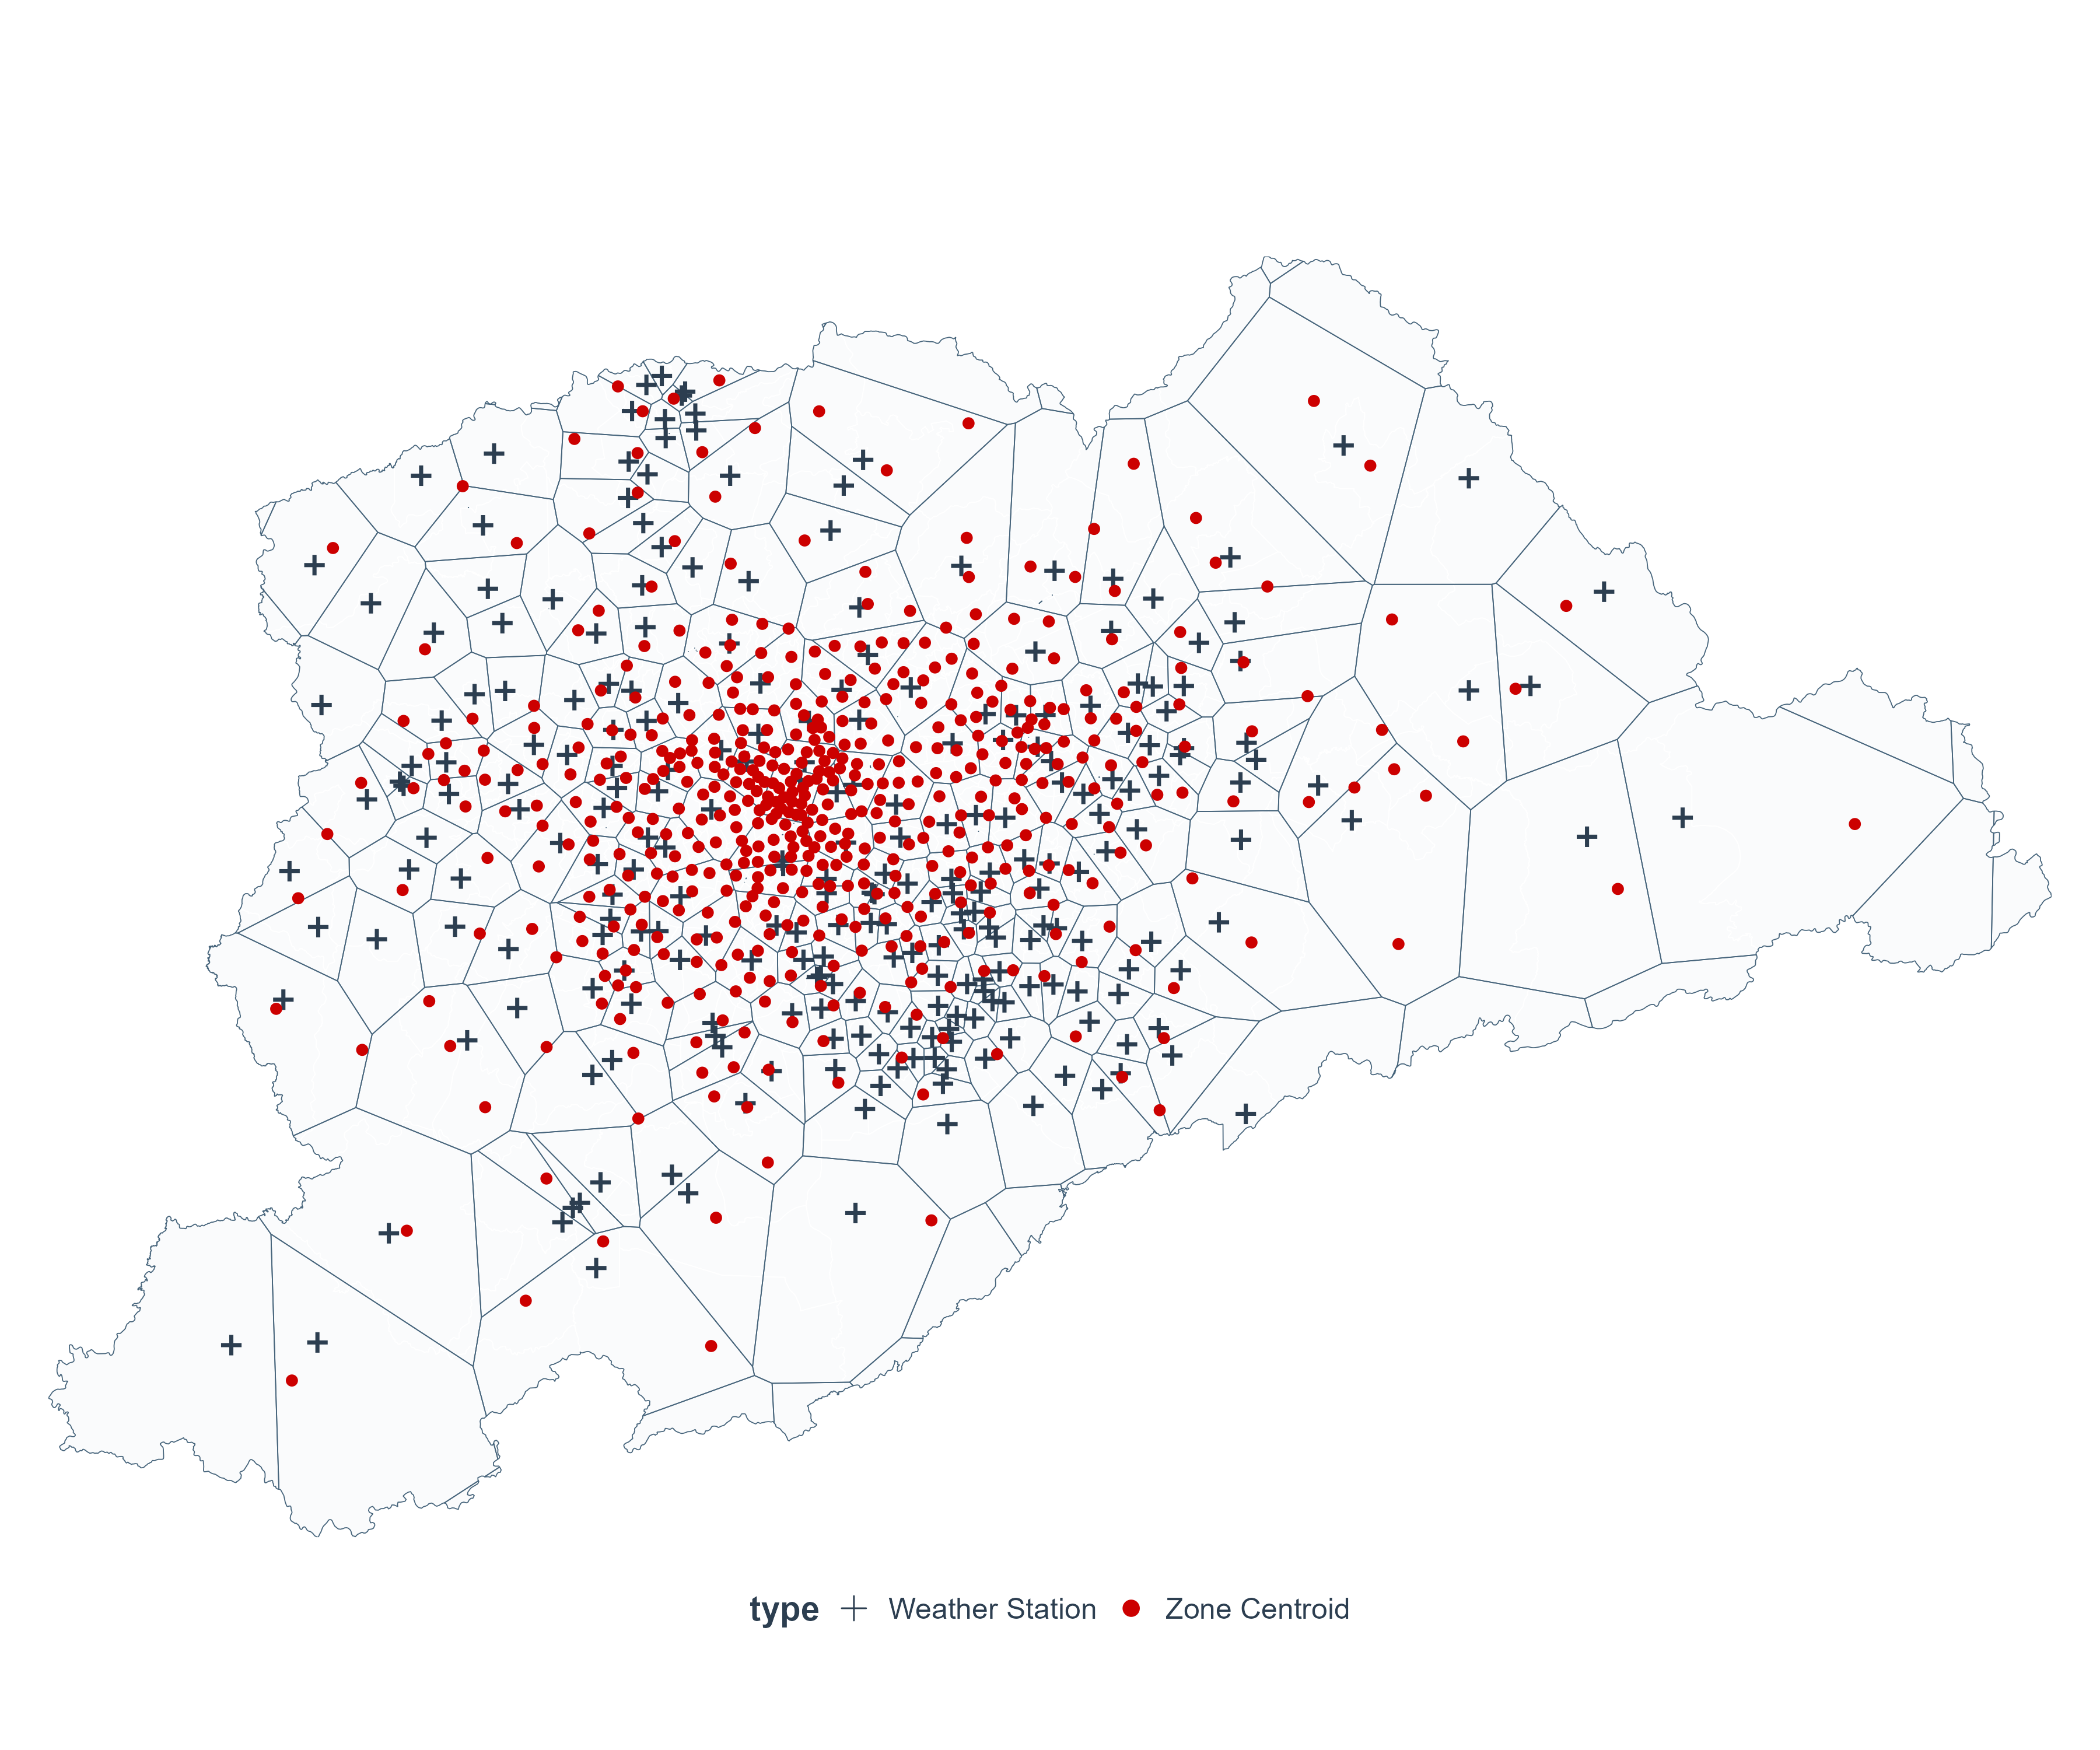
\includegraphics[width=0.45\textwidth]{../figures/rmsp_voronoi.png}
    \caption{Spatial representation of the RMSP region: (left) base map with zone centroids, (right) Voronoi diagram illustrating spatial partitions based on proximity to weather stations.}
    \label{fig:rmsp_voronoi}
\end{figure}
